%%%%%%%%%%%%%%%%%%%%%%%%%%%%%%%%%%%%%%%%%
% University/School Laboratory Report
% LaTeX Template
% Version 4.0 (March 21, 2022)
%
% This template originates from:
% https://www.LaTeXTemplates.com
%
% Authors:
% Vel (vel@latextemplates.com)
% Linux and Unix Users Group at Virginia Tech Wiki
%
% License:
% CC BY-NC-SA 4.0 (https://creativecommons.org/licenses/by-nc-sa/4.0/)
%
%%%%%%%%%%%%%%%%%%%%%%%%%%%%%%%%%%%%%%%%%

%----------------------------------------------------------------------------------------
%	PACKAGES AND DOCUMENT CONFIGURATIONS
%----------------------------------------------------------------------------------------

\documentclass[
	letterpaper, % Paper size, specify a4paper (A4) or letterpaper (US letter)
	10pt, % Default font size, specify 10pt, 11pt or 12pt
]{CSUniSchoolLabReport}

\addbibresource{sample.bib} % Bibliography file (located in the same folder as the template)
%----------------------------------------------------------------------------------------
%	REPORT INFORMATION
%----------------------------------------------------------------------------------------
\usepackage{array}
\usepackage{pdfpages}
\title{Experiment Number 8\\ EP3290} % Report title

\author{Chaganti Kamaraja Siddhartha\\EP20B012} % Author name(s), add additional authors like: '\& James \textsc{Smith}'

\date{\today} % Date of the report

%----------------------------------------------------------------------------------------

\begin{document}

\maketitle % Insert the title, author and date using the information specified above

\begin{center}
	\begin{tabular}{l r}
		Date Performed: & September 6, 2022 \\ % Date the experiment was performed
	\end{tabular}
\end{center}

% If you need to include an abstract, uncomment the lines below
%\begin{abstract}
%	Abstract text
%\end{abstract}

%----------------------------------------------------------------------------------------
%	OBJECTIVE
%----------------------------------------------------------------------------------------
\section{Aim}
To measure the wave length of microwaves by LLOYD'S MIRROR METHOD. 
\section{Components Required}
\begin{enumerate}
	\item Microwave transmitter
	\item Receiver
	\item Metal reflector 
	\item oscilloscope
	\item Connecting probes
\end{enumerate}
\section{Lloyd's mirror method}
\begin{figure}[H] % [H] forces the figure to be placed exactly where it appears in the text
	\centering % Horizontally center the figure
	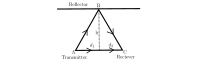
\includegraphics[width=1\textwidth]{l} % Include the figure
	\caption{Lloyd's Mirror setup}
\end{figure}
\begin{enumerate}
	\item The microwave travels directly between the points A and C. 
	\item Also part of the wave gets reflected at B and interferes at C with the original wave. 
	\item A microwave signal is detected when two waves reach the detector in phase
	\item The above setup is called Lloyd's mirror. 
\end{enumerate}
\section{Procedure}
\begin{enumerate}
	\item Arrange the receiver and transmitter at least 1m apart and place a metal reflector such that is located at a point B as shown in the diagram. 
	\item Tabulate the values by slowly moving the metal reflector perpendicular to the transmitter-receiver part and taking down the distances at which minima and maxima occurs. 
	\item Let us consider the initially the mirror is at h1 cm from the center line and next minima occur at h2. 

\end{enumerate}
\vspace{1cm}
\fbox{
\parbox{\textwidth}{

Initial path length (ABC) = \(\sqrt{h_1 ^2 + d_1 ^2}+\sqrt{h_1 ^2 + d_2 ^2}  \) \\
Path length for \(h_2\)  =  \(\sqrt{h_2 ^2 + d_1 ^2}+\sqrt{h_2 ^2 + d_2 ^2}  \) \\
When the difference between the above two path lengths is \(\lambda\), we get minima at both \(h_1\) and \(h_2\).\\ 
Hence, wavelength\\
\[
	\lambda = \sqrt{h_2 ^2 + d_1 ^2}+\sqrt{h_2 ^2 + d_2 ^2} - \sqrt{h_1 ^2 + d_1 ^2}+\sqrt{h_1 ^2 + d_2 ^2}  
\]
}}
\section{Observations}
\begin{center}
	\begin{tabular}{ | m{1cm} | m{3cm}| m{3cm} | } 
		\hline
		S.No	&	\(Distance (mm)\)	&	\(Voltage (V)\) \\
		\hline
		1&5&14\\
2&5.1&13.6\\
3&5.2&13.9\\
4&5.3&13.8\\
5&5.4&14.2\\
6&5.5&14.1\\
7&5.6&14.1\\
8&5.7&13.9\\
9&5.8&13.8\\
10&5.9&13.8\\
11&6&13.8\\
12&6.1&13.8\\
13&6.2&13.6\\
14&6.3&13.4\\
15&6.4&13.2\\
16&6.5&13.4\\
17&6.6&13.6\\
18&6.7&13.4\\
19&6.8&13.2\\
20&6.9&13\\
21&7&12.8\\
22&7.1&12.4\\
23&7.2&12\\
24&7.3&11.8\\
25&7.4&11.4\\
26&7.5&11.2\\
27&7.6&10.6\\
28&7.7&10.4\\
29&7.8&10.2\\
30&7.9&9.7\\
31&8&9.5\\
32&8.1&9.3\\
33&8.2&9.2\\
34&8.3&9.1\\
35&8.4&8.9\\
36&8.5&9.3\\
37&8.6&9.4\\
38&8.7&9.5\\
39&8.8&9.7\\
40&8.9&10.2\\
\hline
	\end{tabular}
\end{center}
\begin{center}
	\begin{tabular}{ | m{1cm} | m{3cm}| m{3cm} | } 
		\hline
		S.No	&	\(Distance (mm)\)	&	\(Voltage (V)\) \\
		\hline

41&9&10.3\\
42&9.1&10.8\\
43&9.2&11\\
44&9.3&11.2\\
45&9.4&11.4\\
46&9.5&11.6\\
47&9.6&11.7\\
48&9.7&11.5\\
49&9.8&11.4\\
50&9.9&11.3\\
51&10&10.6\\
52&10.1&11.2\\
53&10.2&11.1\\
54&10.3&11.2\\
55&10.4&10.9\\
56&10.5&10.6\\
57&10.6&10.8\\
58&10.7&11.3\\
59&10.8&10.8\\
60&10.9&11.2\\
61&11&11.4\\
62&11.1&11.8\\
63&11.2&12\\
64&11.3&12.6\\
65&11.4&12.8\\
66&11.5&12.6\\
67&11.6&12.4\\
68&11.7&12.6\\
69&11.8&12.8\\
70&11.9&12.6\\
71&12&12.4\\
72&12.1&12.2\\
73&12.2&11.8\\
74&12.3&11.4\\
75&12.4&10.4\\
76&12.5&10.3\\
77&12.6&10.2\\
78&12.7&10.4\\
79&12.8&10.4\\
80&12.9&10.2\\
81&13&10.1\\
82&13.1&10.1\\
83&13.2&9.7\\
84&13.3&10.3\\
85&13.4&10.6\\
\hline
	\end{tabular}
\end{center}
\begin{center}
	\begin{tabular}{ | m{1cm} | m{3cm}| m{3cm} | } 
		\hline
		S.No	&	\(Distance (mm)\)	&	\(Voltage (V)\) \\
		\hline
86&13.5&10.8\\
87&13.6&10.9\\
88&13.7&11\\
89&13.8&11.1\\
90&13.9&11.6\\
91&14&12\\
92&14.1&12.2\\
93&14.2&12.4\\
94&14.3&12.5\\
95&14.4&12.2\\
96&14.5&12.2\\
97&14.6&11.8\\
98&14.7&11.4\\
99&14.8&11\\
100&14.9&10.6\\
101&15&10.8\\
102&15.1&10.6\\
103&15.2&10.2\\
104&15.3&10.6\\
105&15.4&10.7\\
106&15.5&10.4\\
107&15.6&10.1\\
108&15.7&9.7\\
109&15.8&9.9\\
110&15.9&10\\
111&16&10.2\\
112&16.1&10.3\\
113&16.2&10.4\\
114&16.3&10.6\\
115&16.4&10.8\\
116&16.5&11.5\\
117&16.6&12.2\\
118&16.7&12.4\\
119&16.8&11.6\\
120&16.9&11.6\\
121&17&11.7\\
122&17.1&11.4\\
123&17.2&10.9\\
124&17.3&10.6\\
125&17.4&10.4\\
126&17.5&10\\
127&17.6&10.4\\
128&17.7&10.6\\
129&17.8&10.2\\
130&17.9&10.4\\
131&18&10.6\\
\hline
	\end{tabular}
\end{center}
\section{Calculations}
\subsection{Finding wavelength}
\section{Advantages}
\begin{enumerate}
	\item The above method is extremely flexible i.e., they do not require proper set up positions. 
	\item The above method is very quick .We can easily find the wavelength of microwaves in a
	matter of minutes. 
\end{enumerate}
\section{Sources of Errors}
\begin{enumerate}
	\item The microwaves diverge a lot. Hence, it is very difficult to detect high output amplitudes.
	Therefore, any external noise gives errors to the measurements. 
	\item Human body is a good absorber of microwaves. Hence, even while doing experiment we could
	accidentally cause error. 
\end{enumerate}
\section{Conclusions}
Thus the wavelength of microwaves is calculated. 
\[
	\boxed{\text{LlOYD'S mirror method } \lambda = }
\]
\end{document}
